% This template originates from the Cambridge University thesis 
% which is created by Prof Harish Bhanderi.  
% This is template follows the GNU license for Education and training
% purposes. (http://www-h.eng.cam.ac.uk/help/tpl/textprocessing/ThesisStyle/) 
% 
%
% I modified for uses in University of Information Technology 
% Vietnam National University. 

\documentclass[oneside,12pt]{Classes/uitBA}


 \ifpdf
     \pdfinfo { /Title  (Thesis title)
                /Creator (TeX)
                /Producer (pdfTeX)
                /Author (Nguyen Van X, Nguyen Van Y)
                /CreationDate (D:20121211000000)  %format D:YYYYMMDDhhmmss
                /ModDate (D:20030815213532)
                /Subject (Thesis title)
                /Keywords (PhD, Thesis)}
     \pdfcatalog { /PageMode (/UseOutlines)
                   /OpenAction (fitbh)  }
 \fi
     
  \university{{ĐẠI HỌC QUỐC GIA THÀNH PHỐ HỒ CHÍ MINH\\
               ĐẠI HỌC CÔNG NGHỆ THÔNG TIN}}
  \collegeordept{{KHOA MẠNG MÁY TÍNH \& TRUYỀN THÔNG}}  
  \degree{KỸ SƯ CÔNG NGHỆ THÔNG TIN}   
  \title{TÊN ĐỀ KHOÁ LUẬN TỐT NGHIỆP KỸ SƯ CNTT} 
  \crest{
\includegraphics[scale=.30]{UITLogo}} 
  \supervisor{{TS. NGUYỄN VĂN XYZ}}
  \author{{NGUYỄN VĂN X - 0123456789 
           \\NGUYỄN VĂN Y - 0123456788}}   
  \degreedate{3, 2013} 
\hbadness=10000
\hfuzz=50pt
\usepackage{StyleFiles/watermark}
\onehalfspacing

\begin{document}
\maketitle
\setcounter{secnumdepth}{3}
\setcounter{tocdepth}{3}

\frontmatter % book mode only
\pagenumbering{roman}
 
\begin{dedication}  

Xin dành tặng quyển luận văn này cho ... 

\end{dedication}

 
 
 
\begin{acknowledgements}      

Tôi xin chân thành cám ơn ... 

\end{acknowledgements}
  
 
\begin{abstracts}         
Tóm tắt luận văn. Tóm tắt luận văn. Tóm tắt luận văn. Tóm tắt luận văn. Tóm tắt luận văn. Tóm tắt luận văn. Tóm tắt luận văn. Tóm tắt luận văn. Tóm tắt luận văn. Tóm tắt luận văn. Tóm tắt luận văn. Tóm tắt luận văn. Tóm tắt luận văn. Tóm tắt luận văn. Tóm tắt luận văn. Tóm tắt luận văn. Tóm tắt luận văn. Tóm tắt luận văn. 

Tóm tắt luận văn. Tóm tắt luận văn. Tóm tắt luận văn. Tóm tắt luận văn. Tóm tắt luận văn. Tóm tắt luận văn. Tóm tắt luận văn. Tóm tắt luận văn. 

Tóm tắt luận văn. Tóm tắt luận văn. Tóm tắt luận văn. Tóm tắt luận văn. Tóm tắt luận văn. Tóm tắt luận văn. Tóm tắt luận văn. Tóm tắt luận văn. Tóm tắt luận văn. Tóm tắt luận văn. Tóm tắt luận văn. Tóm tắt luận văn. Tóm tắt luận văn. Tóm tắt luận văn. Tóm tắt luận văn. Tóm tắt luận văn. 



\end{abstracts}
 

\tableofcontents
\listoffigures
 \printnomenclature  
 \addcontentsline{toc}{chapter}{Nomenclature}

\mainmatter  
% \pagebreak[4]
% \hspace*{1cm}
% \pagebreak[4]
% \hspace*{1cm}
% \pagebreak[4]

\chapter{Đây là chương 1 }
\ifpdf
    \graphicspath{{Chapter1/Chapter1Figs/PNG/}{Chapter1/Chapter1Figs/PDF/}{Chapter1/Chapter1Figs/}}
\else
    \graphicspath{{Chapter1/Chapter1Figs/EPS/}{Chapter1/Chapter1Figs/}}
\fi

\section{Section đầu tiên}
Viết luận văn bằng  \hologo{LaTeX}. Viết luận văn bằng  \hologo{LaTeX}. Viết luận văn bằng  \hologo{LaTeX}. Viết luận văn bằng  \hologo{LaTeX}. Viết luận văn bằng  \hologo{LaTeX}. Viết luận văn bằng  \hologo{LaTeX}. Viết luận văn bằng  \hologo{LaTeX}. Viết luận văn bằng  \hologo{LaTeX}. Viết luận văn bằng  \hologo{LaTeX}. Viết luận văn bằng  \hologo{LaTeX}. Viết luận văn bằng  \hologo{LaTeX}. Viết luận văn bằng  \hologo{LaTeX}. Viết luận văn bằng  \hologo{LaTeX}. Viết luận văn bằng  \hologo{LaTeX}. Viết luận văn bằng  \hologo{LaTeX}. Viết luận văn bằng  \hologo{LaTeX}. Viết luận văn bằng  \hologo{LaTeX}. Viết luận văn bằng  \hologo{LaTeX}. Viết luận văn bằng  \hologo{LaTeX}. Viết luận văn bằng  \hologo{LaTeX}. Viết luận văn bằng  \hologo{LaTeX}.  

Thử nghiệm trích dẫn \cite{Andress2002WLANSecurity}. Trích dẫn tên tác giả \citet{Barbeau2012P2PvoiceOverAdHocSurvey} 
Trích dẫn toàn bộ các tác giả \citet*{Bennett2012MobileDeviceForensicsChallenges}. 

Viết luận văn bằng  \hologo{LaTeX}. Viết luận văn bằng  \hologo{LaTeX}. Viết luận văn bằng  \hologo{LaTeX}. Viết luận văn bằng  \hologo{LaTeX}. Viết luận văn bằng  \hologo{LaTeX}. Viết luận văn bằng  \hologo{LaTeX}. Viết luận văn bằng  \hologo{LaTeX}. Viết luận văn bằng  \hologo{LaTeX}. Viết luận văn bằng  \hologo{LaTeX}. Viết luận văn bằng  \hologo{LaTeX}. Viết luận văn bằng  \hologo{LaTeX}. Viết luận văn bằng  \hologo{LaTeX}. Viết luận văn bằng  \hologo{LaTeX}. Viết luận văn bằng  \hologo{LaTeX}. Viết luận văn bằng  \hologo{LaTeX}. Viết luận văn bằng  \hologo{LaTeX}. Viết luận văn bằng  \hologo{LaTeX}. Viết luận văn bằng  \hologo{LaTeX}. Viết luận văn bằng  \hologo{LaTeX}. Viết luận văn bằng  \hologo{LaTeX}. Viết luận văn bằng  \hologo{LaTeX}. Viết luận văn bằng  \hologo{LaTeX}. Viết luận văn bằng  \hologo{LaTeX}. Viết luận văn bằng  \hologo{LaTeX}. Viết luận văn bằng  \hologo{LaTeX}. Viết luận văn bằng  \hologo{LaTeX}. Viết luận văn bằng  \hologo{LaTeX}. Viết luận văn bằng  \hologo{LaTeX}. Viết luận văn bằng  \hologo{LaTeX}. Viết luận văn bằng  \hologo{LaTeX}. 
Thử nghiệm trích dẫn \citep{Bertino2009LAAandACC}. Trích dẫn tên tác giả \citet{Breu2004TowardsASystemmaticDevelopmentOfSecureSystems} 
Trích dẫn toàn bộ các tác giả \citet*{bunting2012encase}. 


Viết luận văn bằng  \hologo{LaTeX}. Viết luận văn bằng  \hologo{LaTeX}. Viết luận văn bằng  \hologo{LaTeX}. Viết luận văn bằng  \hologo{LaTeX}. Viết luận văn bằng  \hologo{LaTeX}. Viết luận văn bằng  \hologo{LaTeX}. Viết luận văn bằng  \hologo{LaTeX}. Viết luận văn bằng  \hologo{LaTeX}. Viết luận văn bằng  \hologo{LaTeX}. Viết luận văn bằng  \hologo{LaTeX}. Viết luận văn bằng  \hologo{LaTeX}. Viết luận văn bằng  \hologo{LaTeX}. Viết luận văn bằng  \hologo{LaTeX}. Viết luận văn bằng  \hologo{LaTeX}. Viết luận văn bằng  \hologo{LaTeX}. Viết luận văn bằng  \hologo{LaTeX}. Viết luận văn bằng  \hologo{LaTeX}. Viết luận văn bằng  \hologo{LaTeX}. Viết luận văn bằng  \hologo{LaTeX}. Viết luận văn bằng  \hologo{LaTeX}. Viết luận văn bằng  \hologo{LaTeX}. Viết luận văn bằng  \hologo{LaTeX}. Viết luận văn bằng  \hologo{LaTeX}. Viết luận văn bằng  \hologo{LaTeX}. Viết luận văn bằng  \hologo{LaTeX}. Viết luận văn bằng  \hologo{LaTeX}. Viết luận văn bằng  \hologo{LaTeX}. Viết luận văn bằng  \hologo{LaTeX}. Viết luận văn bằng  \hologo{LaTeX}. Viết luận văn bằng  \hologo{LaTeX}. Viết luận văn bằng  \hologo{LaTeX}. Viết luận văn bằng  \hologo{LaTeX}. Viết luận văn bằng  \hologo{LaTeX}. 


Viết luận văn bằng  \hologo{LaTeX}. Viết luận văn bằng  \hologo{LaTeX}. Viết luận văn bằng  \hologo{LaTeX}. Viết luận văn bằng  \hologo{LaTeX}. Viết luận văn bằng  \hologo{LaTeX}. Viết luận văn bằng  \hologo{LaTeX}. Viết luận văn bằng  \hologo{LaTeX}. Viết luận văn bằng  \hologo{LaTeX}. Viết luận văn bằng  \hologo{LaTeX}. Viết luận văn bằng  \hologo{LaTeX}. Viết luận văn bằng  \hologo{LaTeX}. Viết luận văn bằng  \hologo{LaTeX}. Viết luận văn bằng  \hologo{LaTeX}. Viết luận văn bằng  \hologo{LaTeX}. Viết luận văn bằng  \hologo{LaTeX}. Viết luận văn bằng  \hologo{LaTeX}. Viết luận văn bằng  \hologo{LaTeX}. Viết luận văn bằng  \hologo{LaTeX}. Viết luận văn bằng  \hologo{LaTeX}. Viết luận văn bằng  \hologo{LaTeX}. Viết luận văn bằng  \hologo{LaTeX}. 


Thử nghiệm trích dẫn \cite{Ahamed2010FTMforPervasiveEnvironments}. Trích dẫn tên tác giả \citet{Ahamed2010FTMforPervasiveEnvironments}. Trích dẫn đầy đủ 
\citet*{Ahamed2010FTMforPervasiveEnvironments}. 

Để học thêm về cách sử dụng gói trích dẫn natbib, các bạn cần đọc thêm tại đây: http://casa.colorado.edu/\~danforth/comp/tex/tutorial.html

Here is an equation\footnote{the notation is explained in the nomenclature section :-)}:
\begin{eqnarray}
CIF: \hspace*{5mm}F_0^j(a) &=& \frac{1}{2\pi \iota} \oint_{\gamma} \frac{F_0^j(z)}{z - a} dz
\end{eqnarray}
\nomenclature[zcif]{$CIF$}{Cauchy's Integral Formula}                                % first letter Z is for Acronyms 
\nomenclature[aF]{$F$}{complex function}                                                   % first letter A is for Roman symbols
\nomenclature[gp]{$\pi$}{ $\simeq 3.14\ldots$}                                             % first letter G is for Greek Symbols
\nomenclature[gi]{$\iota$}{unit imaginary number $\sqrt{-1}$}                      % first letter G is for Greek Symbols
\nomenclature[gg]{$\gamma$}{a simply closed curve on a complex plane}  % first letter G is for Greek Symbols
\nomenclature[xi]{$\oint_\gamma$}{integration around a curve $\gamma$} % first letter X is for Other Symbols
\nomenclature[rj]{$j$}{superscript index}                                                       % first letter R is for superscripts
\nomenclature[s0]{$0$}{subscript index}                                                        % first letter S is for subscripts

\section{Section  tiếp theo}
 

\subsection{Đây là subsection }
\subsubsection{Đây là sunsubsection }
 
Hạn chế dùng đến x.x.x.... 
\subsection{Đây là subsection tiếp theo}
... and some more ...

Now I would like to cite the following: 
and \cite{Rud73}.

I would also like to include a picture ...

\begin{figure}[!htbp]
  \begin{center}
    \leavevmode
    \ifpdf
      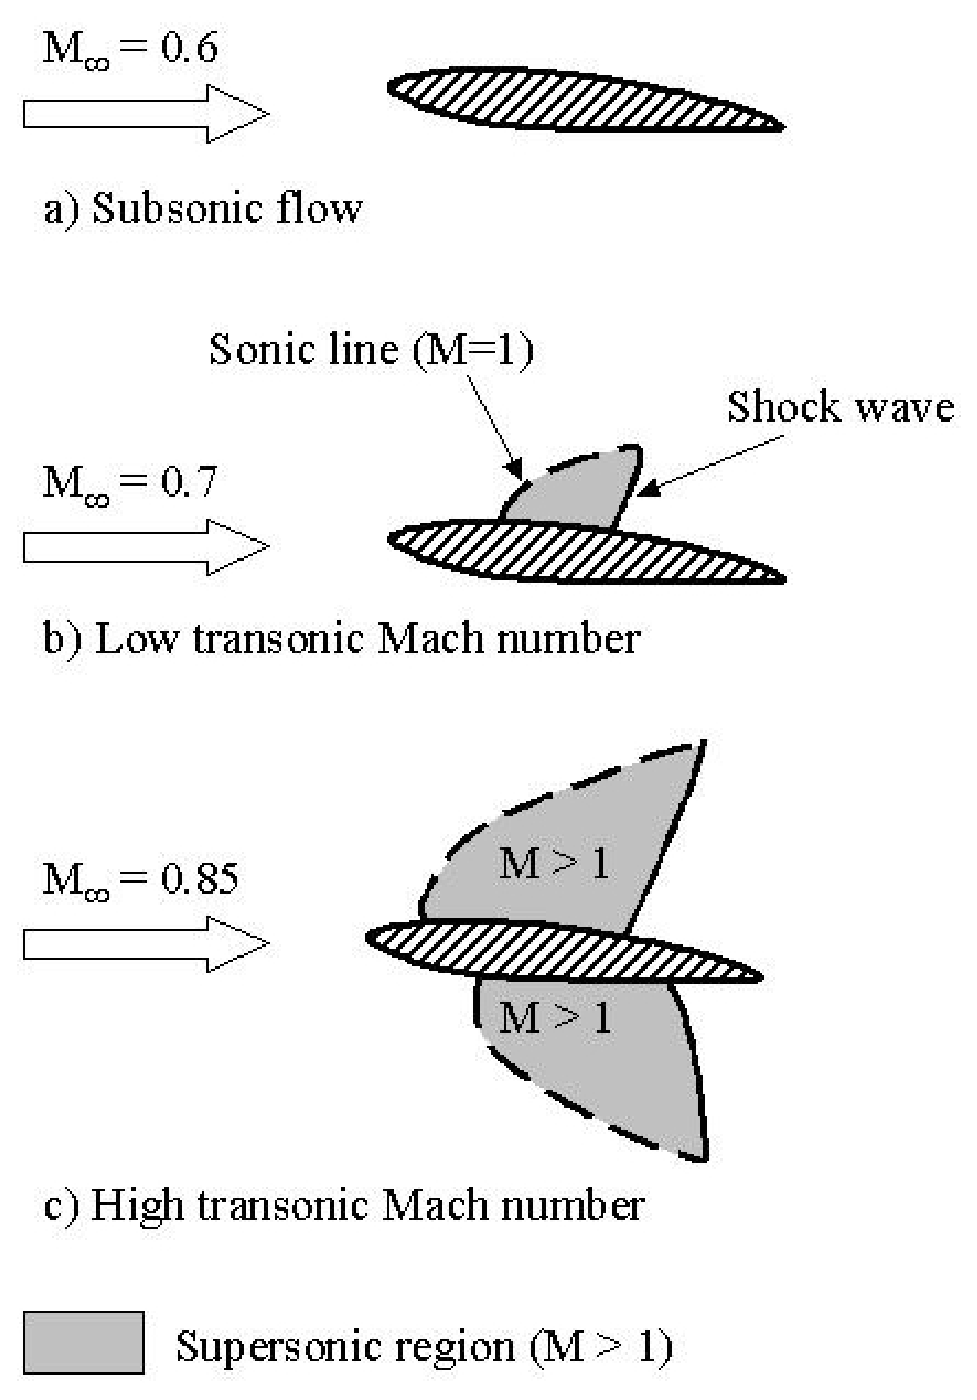
\includegraphics[height=6in]{aflow}
    \else
      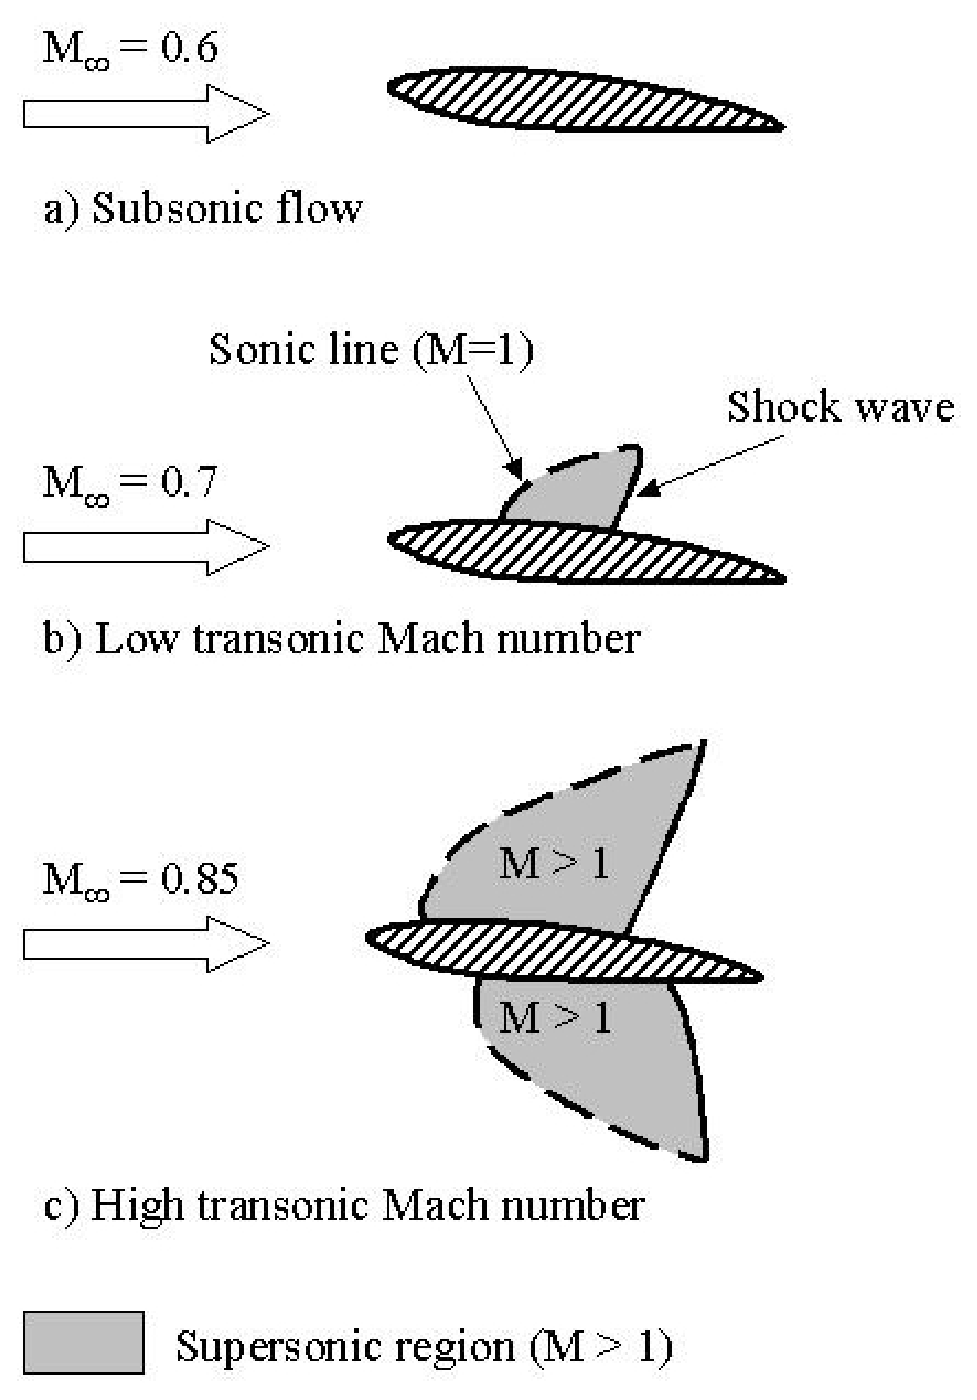
\includegraphics[bb = 92 86 545 742, height=6in]{aflow}
    \fi
    \caption{Airfoil Picture}
    \label{FigAir}
  \end{center}
\end{figure}

% above code has been macro-fied in Classes/MacroFile.tex file
%\InsertFig{\IncludeGraphicsH{aflow}{6in}{92 86 545 742}}{Airfoil Picture}{FigAir}

So as we have now labelled it we can reference it, like so (\ref{FigAir}) and it
is on Page \pageref{FigAir}. And as we can see, it is a very nice picture and we
can talk about it all we want and when we are tired we can move on to the next
chapter ...

I would also like to add an extra bookmark in acroread like so ...
\ifpdf
  \pdfbookmark[2]{bookmark text is here}{And this is what I want bookmarked}
\fi


\section{Kết chương}
Viết luận văn bằng  \hologo{LaTeX}. Viết luận văn bằng  \hologo{LaTeX}. Viết luận văn bằng  \hologo{LaTeX}. Viết luận văn bằng  \hologo{LaTeX}. Viết luận văn bằng  \hologo{LaTeX}. Viết luận văn bằng  \hologo{LaTeX}. Viết luận văn bằng  \hologo{LaTeX}. Viết luận văn bằng  \hologo{LaTeX}. Viết luận văn bằng  \hologo{LaTeX}. Viết luận văn bằng  \hologo{LaTeX}. Viết luận văn bằng  \hologo{LaTeX}. Viết luận văn bằng  \hologo{LaTeX}. Viết luận văn bằng  \hologo{LaTeX}. Viết luận văn bằng  \hologo{LaTeX}. Viết luận văn bằng  \hologo{LaTeX}. Viết luận văn bằng  \hologo{LaTeX}. Viết luận văn bằng  \hologo{LaTeX}. Viết luận văn bằng  \hologo{LaTeX}. Viết luận văn bằng  \hologo{LaTeX}. Viết luận văn bằng  \hologo{LaTeX}. Viết luận văn bằng  \hologo{LaTeX}.  


\chapter{Đây là chương 2}
\ifpdf
    \graphicspath{{Chapter2/Chapter2Figs/PNG/}{Chapter2/Chapter2Figs/PDF/}{Chapter2/Chapter2Figs/}}
\else
    \graphicspath{{Chapter2/Chapter2Figs/EPS/}{Chapter2/Chapter2Figs/}}
\fi

\section{First Section}
\markboth{\MakeUppercase{\thechapter. My Second Chapter }}
Viết luận văn bằng  \hologo{LaTeX}. Viết luận văn bằng  \hologo{LaTeX}. Viết luận văn bằng  \hologo{LaTeX}. Viết luận văn bằng  \hologo{LaTeX}. Viết luận văn bằng  \hologo{LaTeX}. Viết luận văn bằng  \hologo{LaTeX}. Viết luận văn bằng  \hologo{LaTeX}. Viết luận văn bằng  \hologo{LaTeX}. Viết luận văn bằng  \hologo{LaTeX}. Viết luận văn bằng  \hologo{LaTeX}. Viết luận văn bằng  \hologo{LaTeX}. Viết luận văn bằng  \hologo{LaTeX}. Viết luận văn bằng  \hologo{LaTeX}. Viết luận văn bằng  \hologo{LaTeX}. Viết luận văn bằng  \hologo{LaTeX}. Viết luận văn bằng  \hologo{LaTeX}. Viết luận văn bằng  \hologo{LaTeX}. Viết luận văn bằng  \hologo{LaTeX}. Viết luận văn bằng  \hologo{LaTeX}. Viết luận văn bằng  \hologo{LaTeX}. Viết luận văn bằng  \hologo{LaTeX}. 



\section{Second Section}
\markboth{\MakeUppercase{\thechapter. My Second Chapter }}
Viết luận văn bằng  \hologo{LaTeX}. Viết luận văn bằng  \hologo{LaTeX}. Viết luận văn bằng  \hologo{LaTeX}. Viết luận văn bằng  \hologo{LaTeX}. Viết luận văn bằng  \hologo{LaTeX}. Viết luận văn bằng  \hologo{LaTeX}. Viết luận văn bằng  \hologo{LaTeX}. Viết luận văn bằng  \hologo{LaTeX}. Viết luận văn bằng  \hologo{LaTeX}. Viết luận văn bằng  \hologo{LaTeX}. Viết luận văn bằng  \hologo{LaTeX}. Viết luận văn bằng  \hologo{LaTeX}. Viết luận văn bằng  \hologo{LaTeX}. Viết luận văn bằng  \hologo{LaTeX}. Viết luận văn bằng  \hologo{LaTeX}. Viết luận văn bằng  \hologo{LaTeX}. Viết luận văn bằng  \hologo{LaTeX}. Viết luận văn bằng  \hologo{LaTeX}. Viết luận văn bằng  \hologo{LaTeX}. Viết luận văn bằng  \hologo{LaTeX}. Viết luận văn bằng  \hologo{LaTeX}. 


\subsection{first subsection in the Second Section}
... and some more ...
Viết luận văn bằng  \hologo{LaTeX}. Viết luận văn bằng  \hologo{LaTeX}. Viết luận văn bằng  \hologo{LaTeX}. Viết luận văn bằng  \hologo{LaTeX}. Viết luận văn bằng  \hologo{LaTeX}. Viết luận văn bằng  \hologo{LaTeX}. Viết luận văn bằng  \hologo{LaTeX}. Viết luận văn bằng  \hologo{LaTeX}. Viết luận văn bằng  \hologo{LaTeX}. Viết luận văn bằng  \hologo{LaTeX}. Viết luận văn bằng  \hologo{LaTeX}. Viết luận văn bằng  \hologo{LaTeX}. Viết luận văn bằng  \hologo{LaTeX}. Viết luận văn bằng  \hologo{LaTeX}. Viết luận văn bằng  \hologo{LaTeX}. Viết luận văn bằng  \hologo{LaTeX}. Viết luận văn bằng  \hologo{LaTeX}. Viết luận văn bằng  \hologo{LaTeX}. Viết luận văn bằng  \hologo{LaTeX}. Viết luận văn bằng  \hologo{LaTeX}. Viết luận văn bằng  \hologo{LaTeX}. 
\subsection{second subsection in the Second Section}
... and some more ...
Viết luận văn bằng  \hologo{LaTeX}. Viết luận văn bằng  \hologo{LaTeX}. Viết luận văn bằng  \hologo{LaTeX}. Viết luận văn bằng  \hologo{LaTeX}. Viết luận văn bằng  \hologo{LaTeX}. Viết luận văn bằng  \hologo{LaTeX}. Viết luận văn bằng  \hologo{LaTeX}. Viết luận văn bằng  \hologo{LaTeX}. Viết luận văn bằng  \hologo{LaTeX}. Viết luận văn bằng  \hologo{LaTeX}. Viết luận văn bằng  \hologo{LaTeX}. Viết luận văn bằng  \hologo{LaTeX}. Viết luận văn bằng  \hologo{LaTeX}. Viết luận văn bằng  \hologo{LaTeX}. Viết luận văn bằng  \hologo{LaTeX}. Viết luận văn bằng  \hologo{LaTeX}. Viết luận văn bằng  \hologo{LaTeX}. Viết luận văn bằng  \hologo{LaTeX}. Viết luận văn bằng  \hologo{LaTeX}. Viết luận văn bằng  \hologo{LaTeX}. Viết luận văn bằng  \hologo{LaTeX}. 
\subsection{third subsection in the Second Section}
... and some more ...

\section{Kết chương}
Viết luận văn bằng  \hologo{LaTeX}. Viết luận văn bằng  \hologo{LaTeX}. Viết luận văn bằng  \hologo{LaTeX}. Viết luận văn bằng  \hologo{LaTeX}. Viết luận văn bằng  \hologo{LaTeX}. Viết luận văn bằng  \hologo{LaTeX}. Viết luận văn bằng  \hologo{LaTeX}. Viết luận văn bằng  \hologo{LaTeX}. Viết luận văn bằng  \hologo{LaTeX}. Viết luận văn bằng  \hologo{LaTeX}. Viết luận văn bằng  \hologo{LaTeX}. Viết luận văn bằng  \hologo{LaTeX}. Viết luận văn bằng  \hologo{LaTeX}. Viết luận văn bằng  \hologo{LaTeX}. Viết luận văn bằng  \hologo{LaTeX}. Viết luận văn bằng  \hologo{LaTeX}. Viết luận văn bằng  \hologo{LaTeX}. Viết luận văn bằng  \hologo{LaTeX}. Viết luận văn bằng  \hologo{LaTeX}. Viết luận văn bằng  \hologo{LaTeX}. Viết luận văn bằng  \hologo{LaTeX}.  

\chapter{Chương 3}
\ifpdf
    \graphicspath{{Chapter3/Chapter3Figs/PNG/}{Chapter3/Chapter3Figs/PDF/}{Chapter3/Chapter3Figs/}}
\else
    \graphicspath{{Chapter3/Chapter3Figs/EPS/}{Chapter3/Chapter3Figs/}}
\fi

\section{First Section of the Third Chapter}
\markboth{\MakeUppercase{\thechapter. My Third Chapter }}{\thechapter. My Third Chapter}
And now I begin my third chapter here ...

\subsection{first subsection in the First Section}
... and some more 

\subsection{second subsection in the First Section}
... and some more ...

\subsubsection{first subsub section in the second subsection}
... and some more in the first subsub section otherwise it all looks the same
doesn't it? well we can add some text to it ...

\subsection{third subsection in the First Section}
... and some more ...

  Viết luận văn bằng  \hologo{LaTeX}. Viết luận văn bằng  \hologo{LaTeX}. Viết luận văn bằng  \hologo{LaTeX}. Viết luận văn bằng  \hologo{LaTeX}. Viết luận văn bằng  \hologo{LaTeX}. Viết luận văn bằng  \hologo{LaTeX}. Viết luận văn bằng  \hologo{LaTeX}. Viết luận văn bằng  \hologo{LaTeX}. Viết luận văn bằng  \hologo{LaTeX}. Viết luận văn bằng  \hologo{LaTeX}. Viết luận văn bằng  \hologo{LaTeX}. Viết luận văn bằng  \hologo{LaTeX}. Viết luận văn bằng  \hologo{LaTeX}. Viết luận văn bằng  \hologo{LaTeX}. Viết luận văn bằng  \hologo{LaTeX}. Viết luận văn bằng  \hologo{LaTeX}. Viết luận văn bằng  \hologo{LaTeX}. Viết luận văn bằng  \hologo{LaTeX}. Viết luận văn bằng  \hologo{LaTeX}. Viết luận văn bằng  \hologo{LaTeX}. Viết luận văn bằng  \hologo{LaTeX}. 
  
  Viết luận văn bằng  \hologo{LaTeX}. Viết luận văn bằng  \hologo{LaTeX}. Viết luận văn bằng  \hologo{LaTeX}. Viết luận văn bằng  \hologo{LaTeX}. Viết luận văn bằng  \hologo{LaTeX}. Viết luận văn bằng  \hologo{LaTeX}. Viết luận văn bằng  \hologo{LaTeX}. Viết luận văn bằng  \hologo{LaTeX}. Viết luận văn bằng  \hologo{LaTeX}. Viết luận văn bằng  \hologo{LaTeX}. Viết luận văn bằng  \hologo{LaTeX}. Viết luận văn bằng  \hologo{LaTeX}. Viết luận văn bằng  \hologo{LaTeX}. Viết luận văn bằng  \hologo{LaTeX}. Viết luận văn bằng  \hologo{LaTeX}. Viết luận văn bằng  \hologo{LaTeX}. Viết luận văn bằng  \hologo{LaTeX}. Viết luận văn bằng  \hologo{LaTeX}. Viết luận văn bằng  \hologo{LaTeX}. Viết luận văn bằng  \hologo{LaTeX}. Viết luận văn bằng  \hologo{LaTeX}. 
  
  
 
\begin{figure} 
\centering
\subfigure[tui-main]{
   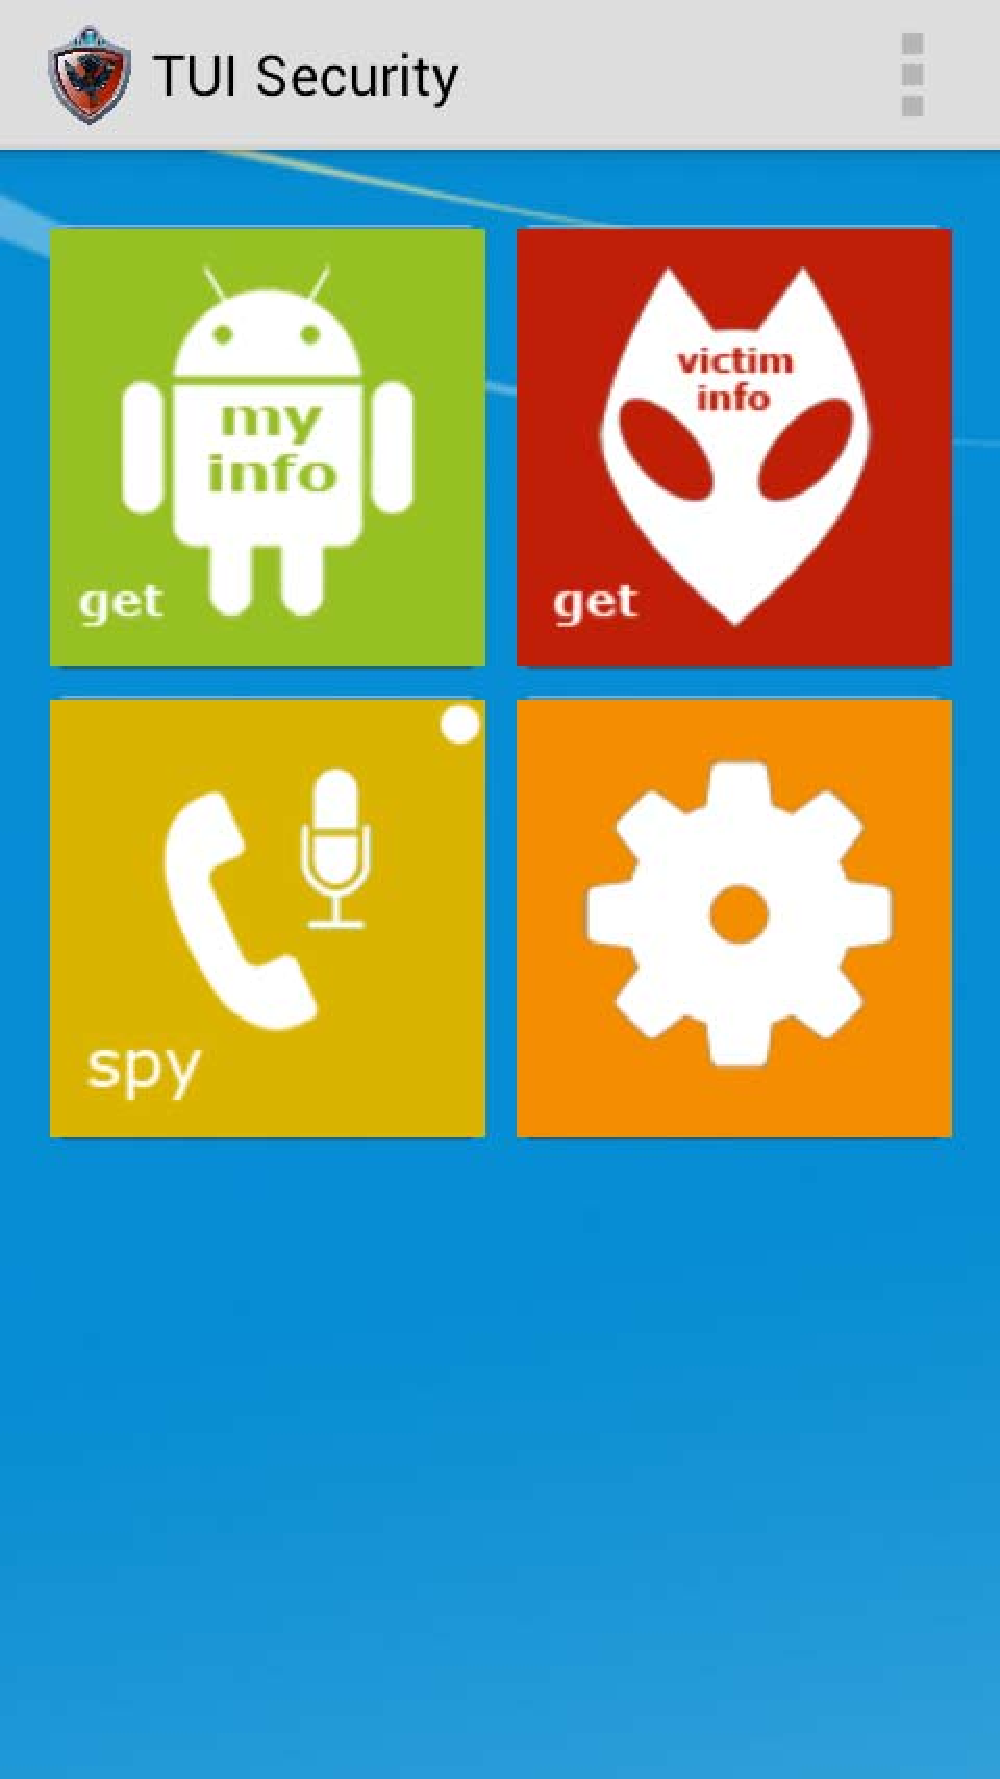
\includegraphics[width=0.30\textwidth] {tui-main.pdf}
   \label{fig:tui-main}}
\subfigure[tui-victim controls]{
   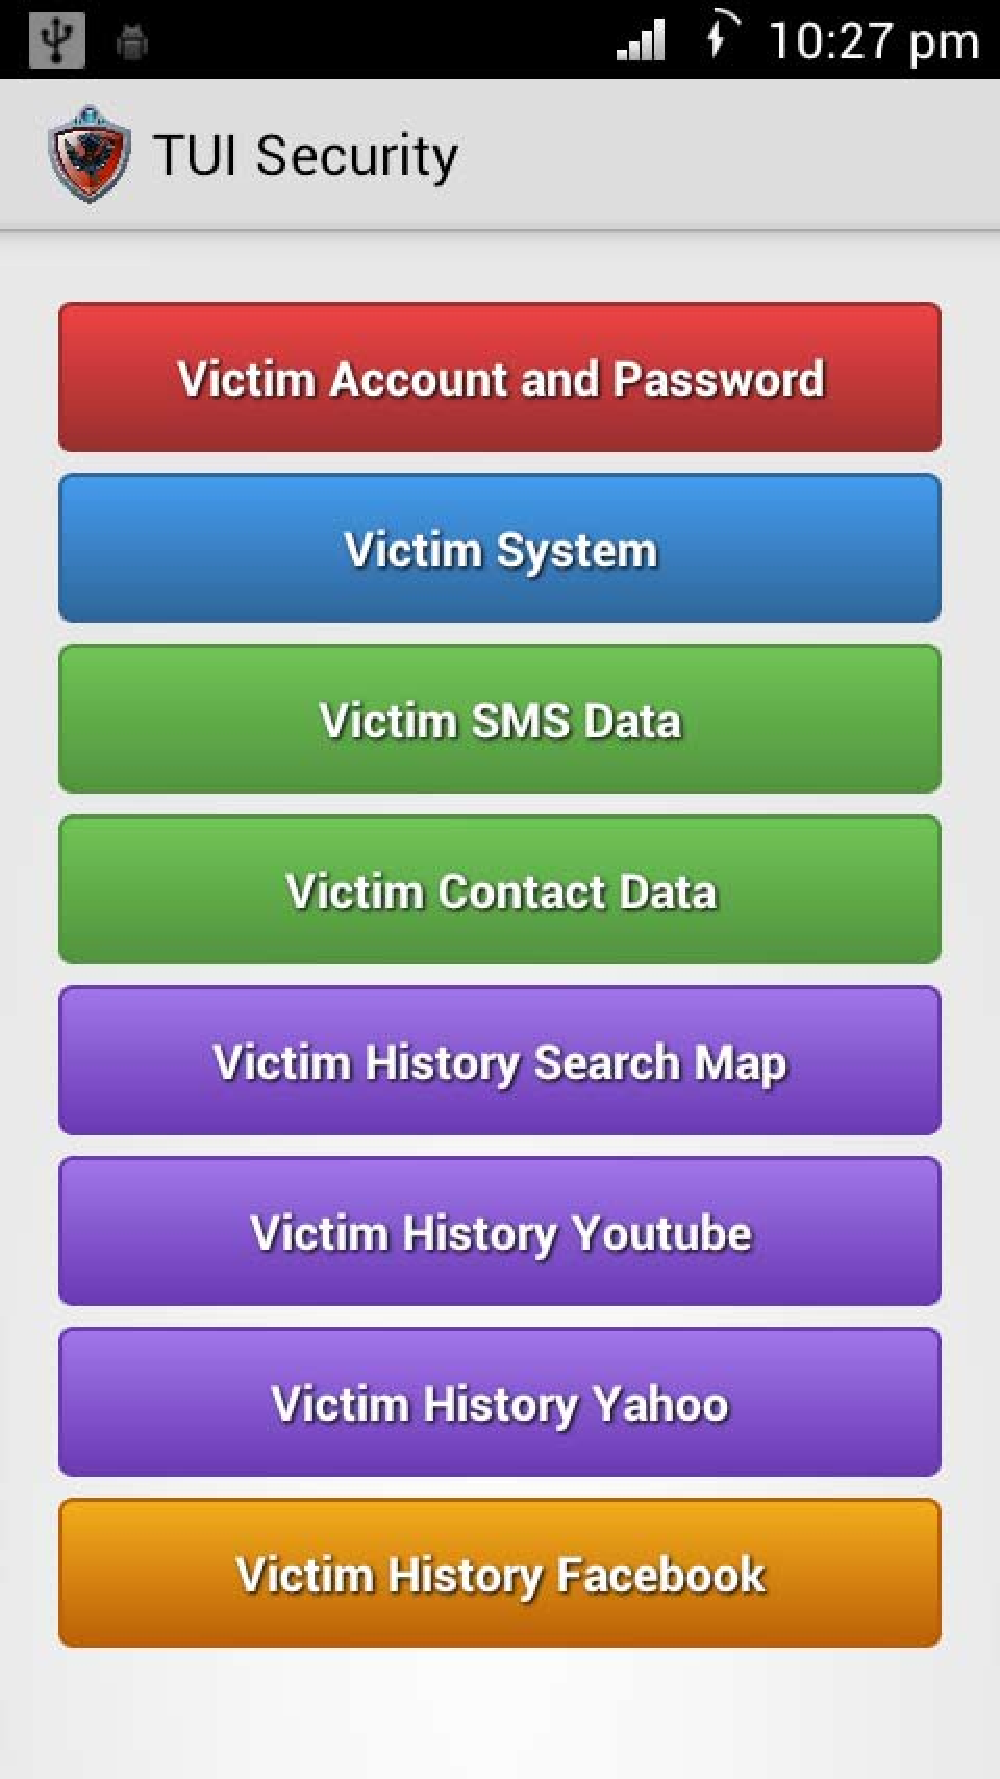
\includegraphics[width=0.30\textwidth] {tui-controls.pdf}
   \label{fig:tui-controls}}
\subfigure[tui-get-phone-info-controls]{
   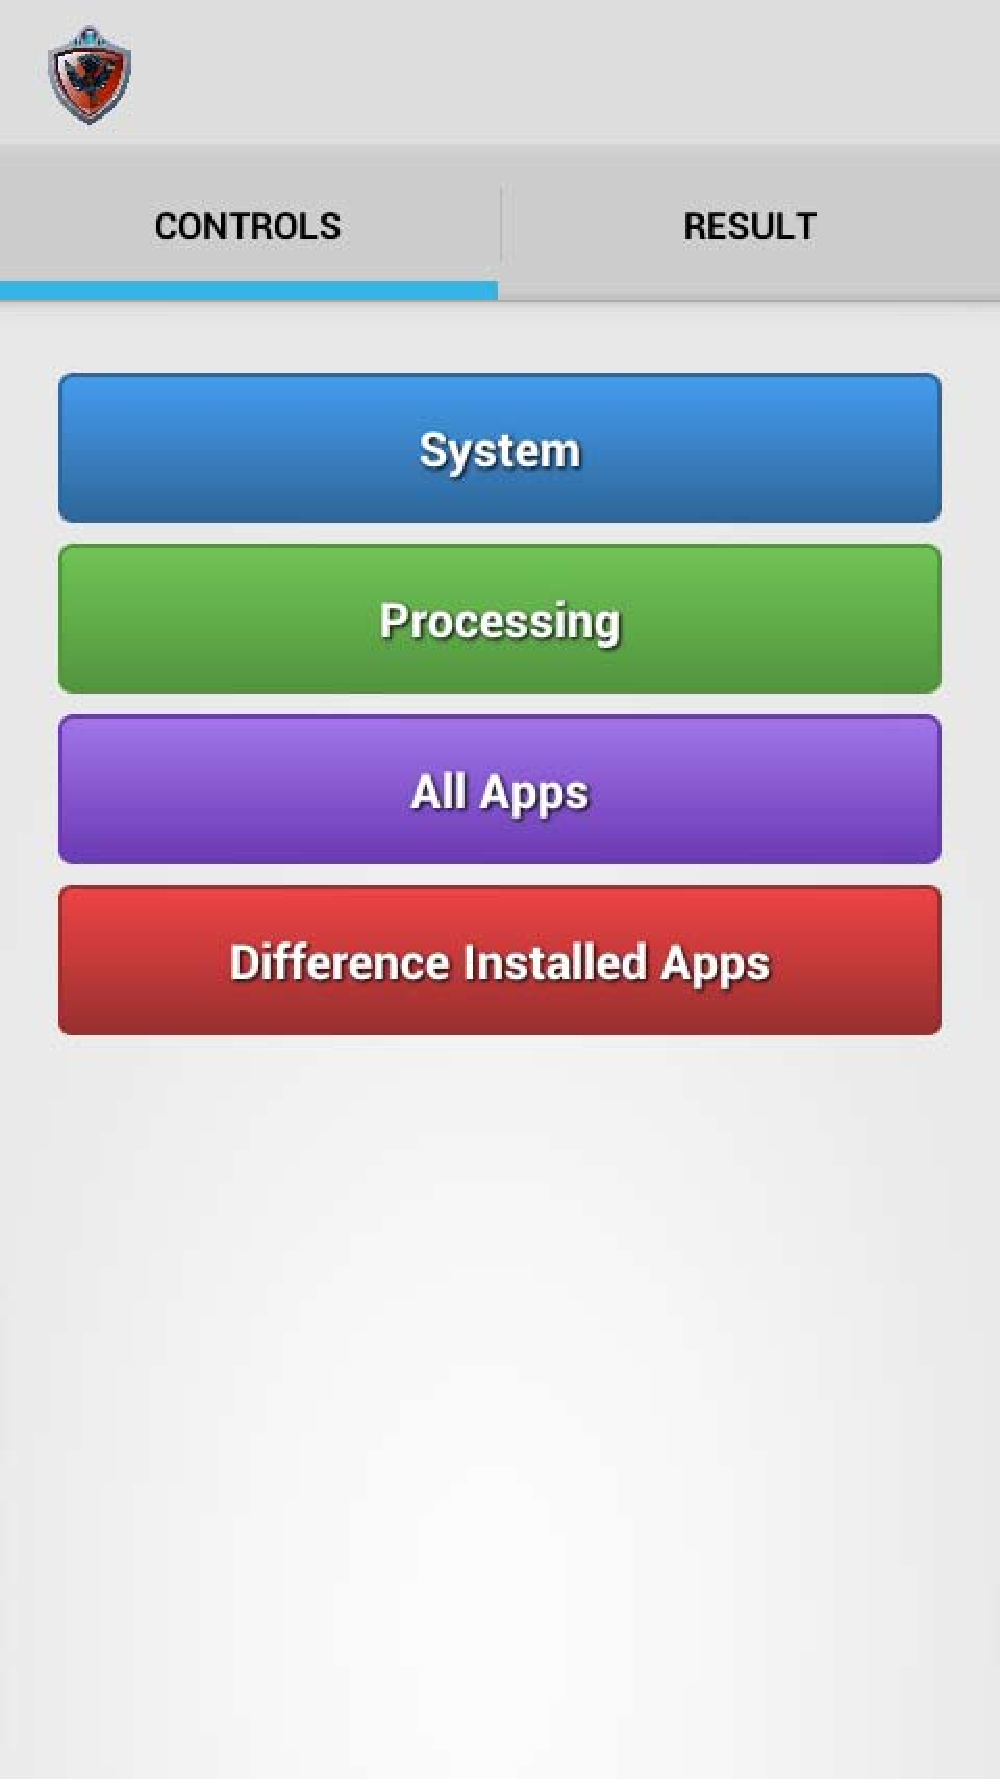
\includegraphics[width=0.30\textwidth] {tui-get-phone-info-controls.pdf}
   \label{fig:tui-get-phone-info-controls}}
\label{myfigure}
\caption{TUI security program main features}
\end{figure}

Viết luận văn bằng  \hologo{LaTeX}. Viết luận văn bằng  \hologo{LaTeX}. Viết luận văn bằng  \hologo{LaTeX}. Viết luận văn bằng  \hologo{LaTeX}. Viết luận văn bằng  \hologo{LaTeX}. Viết luận văn bằng  \hologo{LaTeX}. Viết luận văn bằng  \hologo{LaTeX}. Viết luận văn bằng  \hologo{LaTeX}. Viết luận văn bằng  \hologo{LaTeX}. Viết luận văn bằng  \hologo{LaTeX}. Viết luận văn bằng  \hologo{LaTeX}. Viết luận văn bằng  \hologo{LaTeX}. Viết luận văn bằng  \hologo{LaTeX}. Viết luận văn bằng  \hologo{LaTeX}. Viết luận văn bằng  \hologo{LaTeX}. Viết luận văn bằng  \hologo{LaTeX}. Viết luận văn bằng  \hologo{LaTeX}. Viết luận văn bằng  \hologo{LaTeX}. Viết luận văn bằng  \hologo{LaTeX}. Viết luận văn bằng  \hologo{LaTeX}. Viết luận văn bằng  \hologo{LaTeX}. 

Viết luận văn bằng  \hologo{LaTeX}. Viết luận văn bằng  \hologo{LaTeX}. Viết luận văn bằng  \hologo{LaTeX}. Viết luận văn bằng  \hologo{LaTeX}. Viết luận văn bằng  \hologo{LaTeX}. Viết luận văn bằng  \hologo{LaTeX}. Viết luận văn bằng  \hologo{LaTeX}. Viết luận văn bằng  \hologo{LaTeX}. Viết luận văn bằng  \hologo{LaTeX}. Viết luận văn bằng  \hologo{LaTeX}. Viết luận văn bằng  \hologo{LaTeX}. Viết luận văn bằng  \hologo{LaTeX}. Viết luận văn bằng  \hologo{LaTeX}. Viết luận văn bằng  \hologo{LaTeX}. Viết luận văn bằng  \hologo{LaTeX}. Viết luận văn bằng  \hologo{LaTeX}. Viết luận văn bằng  \hologo{LaTeX}. Viết luận văn bằng  \hologo{LaTeX}. Viết luận văn bằng  \hologo{LaTeX}. Viết luận văn bằng  \hologo{LaTeX}. Viết luận văn bằng  \hologo{LaTeX}. 


 
\subsubsection{first subsub section in the third subsection}
... and some more in the first subsub section otherwise it all looks the same
doesn't it? well we can add some text to it and some more and some more and
some more and some more and some more and some more and some more ...

\subsubsection{second subsub section in the third subsection}
... and some more in the first subsub section otherwise it all looks the same
doesn't it? well we can add some text to it ...

\section{Second Section of the Third Chapter}
\markboth{\MakeUppercase{\thechapter. My Third Chapter }}{\thechapter. My Third Chapter}
and here I write more ...


\section{Kết chương}
Viết luận văn bằng  \hologo{LaTeX}. Viết luận văn bằng  \hologo{LaTeX}. Viết luận văn bằng  \hologo{LaTeX}. Viết luận văn bằng  \hologo{LaTeX}. Viết luận văn bằng  \hologo{LaTeX}. Viết luận văn bằng  \hologo{LaTeX}. Viết luận văn bằng  \hologo{LaTeX}. Viết luận văn bằng  \hologo{LaTeX}. Viết luận văn bằng  \hologo{LaTeX}. Viết luận văn bằng  \hologo{LaTeX}. Viết luận văn bằng  \hologo{LaTeX}. Viết luận văn bằng  \hologo{LaTeX}. Viết luận văn bằng  \hologo{LaTeX}. Viết luận văn bằng  \hologo{LaTeX}. Viết luận văn bằng  \hologo{LaTeX}. Viết luận văn bằng  \hologo{LaTeX}. Viết luận văn bằng  \hologo{LaTeX}. Viết luận văn bằng  \hologo{LaTeX}. Viết luận văn bằng  \hologo{LaTeX}. Viết luận văn bằng  \hologo{LaTeX}. Viết luận văn bằng  \hologo{LaTeX}.  


\def\baselinestretch{1}
\chapter{Kết luận và hướng phát triển}
\ifpdf
    \graphicspath{{Conclusions/ConclusionsFigs/PNG/}{Conclusions/ConclusionsFigs/PDF/}{Conclusions/ConclusionsFigs/}}
\else
    \graphicspath{{Conclusions/ConclusionsFigs/EPS/}{Conclusions/ConclusionsFigs/}}
\fi

\def\baselinestretch{1.66}

Here I put my conclusions ...
Viết luận văn bằng  \hologo{LaTeX}. Viết luận văn bằng  \hologo{LaTeX}. Viết luận văn bằng  \hologo{LaTeX}. Viết luận văn bằng  \hologo{LaTeX}. Viết luận văn bằng  \hologo{LaTeX}. Viết luận văn bằng  \hologo{LaTeX}. Viết luận văn bằng  \hologo{LaTeX}. Viết luận văn bằng  \hologo{LaTeX}. Viết luận văn bằng  \hologo{LaTeX}. Viết luận văn bằng  \hologo{LaTeX}. Viết luận văn bằng  \hologo{LaTeX}. Viết luận văn bằng  \hologo{LaTeX}. Viết luận văn bằng  \hologo{LaTeX}. Viết luận văn bằng  \hologo{LaTeX}. Viết luận văn bằng  \hologo{LaTeX}. Viết luận văn bằng  \hologo{LaTeX}. Viết luận văn bằng  \hologo{LaTeX}. Viết luận văn bằng  \hologo{LaTeX}. Viết luận văn bằng  \hologo{LaTeX}. Viết luận văn bằng  \hologo{LaTeX}. Viết luận văn bằng  \hologo{LaTeX}. 
Viết luận văn bằng  \hologo{LaTeX}. Viết luận văn bằng  \hologo{LaTeX}. Viết luận văn bằng  \hologo{LaTeX}. Viết luận văn bằng  \hologo{LaTeX}. Viết luận văn bằng  \hologo{LaTeX}. Viết luận văn bằng  \hologo{LaTeX}. Viết luận văn bằng  \hologo{LaTeX}. Viết luận văn bằng  \hologo{LaTeX}. Viết luận văn bằng  \hologo{LaTeX}. Viết luận văn bằng  \hologo{LaTeX}. Viết luận văn bằng  \hologo{LaTeX}. Viết luận văn bằng  \hologo{LaTeX}. Viết luận văn bằng  \hologo{LaTeX}. Viết luận văn bằng  \hologo{LaTeX}. Viết luận văn bằng  \hologo{LaTeX}. Viết luận văn bằng  \hologo{LaTeX}. Viết luận văn bằng  \hologo{LaTeX}. Viết luận văn bằng  \hologo{LaTeX}. Viết luận văn bằng  \hologo{LaTeX}. Viết luận văn bằng  \hologo{LaTeX}. Viết luận văn bằng  \hologo{LaTeX}. 

%%% ----------------------------------------------------------------------

% ------------------------------------------------------------------------

%%% Local Variables: 
%%% mode: latex
%%% TeX-master: "../thesis"
%%% End: 


\backmatter  
\appendix
\chapter{Phụ lục A}

Đây là phụ lục A 

% ------------------------------------------------------------------------

%%% Local Variables: 
%%% mode: latex
%%% TeX-master: "../thesis"
%%% End: 

\chapter{Phụ lục B}
Đây là phụ lục B 
% ------------------------------------------------------------------------

%%% Local Variables: 
%%% mode: latex
%%% TeX-master: "../thesis"
%%% End: 

 
\bibliographystyle{Classes/jmb} % bibliography style
\renewcommand{\bibname}{References} % changes default name Bibliography to References
\bibliography{security} % References file

\end{document}
